\documentclass[12pt, a4paper, onecolumn]{IEEEtran}
% https://www.monash.edu/rlo/quick-study-guides/writing-a-case-study
\usepackage{url} % for typesetting URLs
\usepackage{hyperref}
\usepackage{cleveref}
\hypersetup{
	colorlinks=true,
	linkcolor=blue,
	filecolor=blue,
	citecolor=blue,
	urlcolor=magenta,
}
\usepackage[style=ieee]{biblatex}

% Citation Needed Command
\usepackage{xcolor}
\newcommand{\citationneeded}{[\textcolor{blue}{citation needed}]}

\usepackage{caption}
\usepackage{subcaption}
\usepackage{graphicx}
\graphicspath{ {./pictures/} }

%% Bibliography
\addbibresource{./bibliography.bib}

\title{Design of a Variable Amplitude Picking Mechanism}
\author{Joshua Benfell\\Team Members: Jason McCormick, Zach Rogers, Kibra Tesfay}

\begin{document}

	\maketitle
    \section{Introduction}
		Chordophones have been a topic of increasing research interest as a method of automating string instruments.
		These robots are constructed from many subsystems in charge of tasks froms picking the string to selecting the note to play \cite{VUW_Chordophones}.
		This paper focuses on the design of the picking and damping mechanisms of a chordophone robot.
		The picking mechanism will aim to create 3 different volumes of sound and be able to achieve a rate of 120 picks per second.
		The damping mechanism will aim to stop the vibrations in the string within 250 milliseconds.


	\section{Group Decision}
		\begin{figure}[!h]
			\centering
			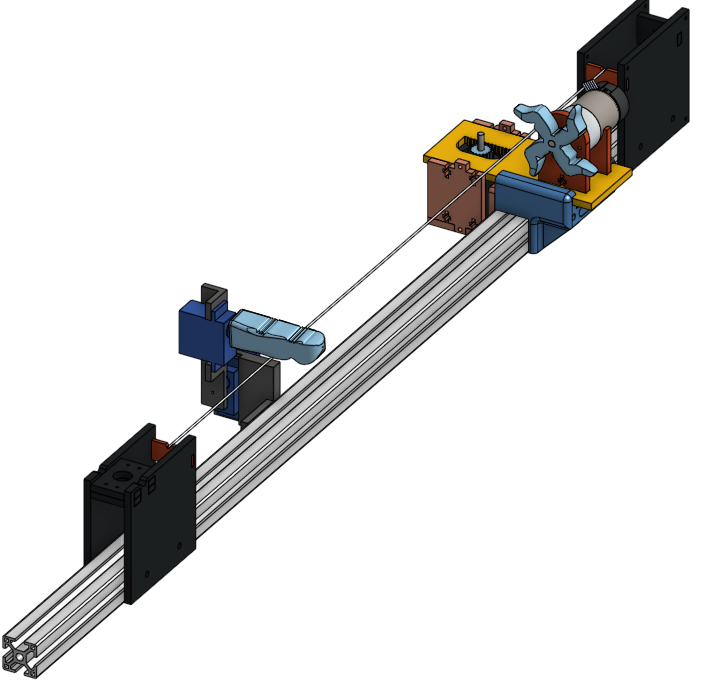
\includegraphics[width=0.5\columnwidth]{chordophoneModel.png}
			\caption{Model of the intended chordophone}
			\label{fig:model}
		\end{figure}
		The desired outcome decided amongst the group was a chordophone that offered material choice.
		The material selected were plastic to mimic a picks sharpness, silicone to mimic the subtleness and flexibility of human skin, and foam as a softer damping material.
		This was decided upon as no prior literature had been found to use a non-standard picking material to pluck the string.

		For the damping mechanism this involved a rotating damping that allowed you to select from the different damping materials listed above.
		For the picking, the intention was a two sided finger, containing some silicone on one side to represent the fleshy side of the finger.
		On the other side was a harder plastic or guitar pick as this represented a nail.
		From this the direction the pick wheel rotated would determine which material was used to pick the string.
		This is all reflected in the model created for the project in \Cref{fig:model}.
		
    \section{Design}
		\begin{figure}[!h]
			\centering
			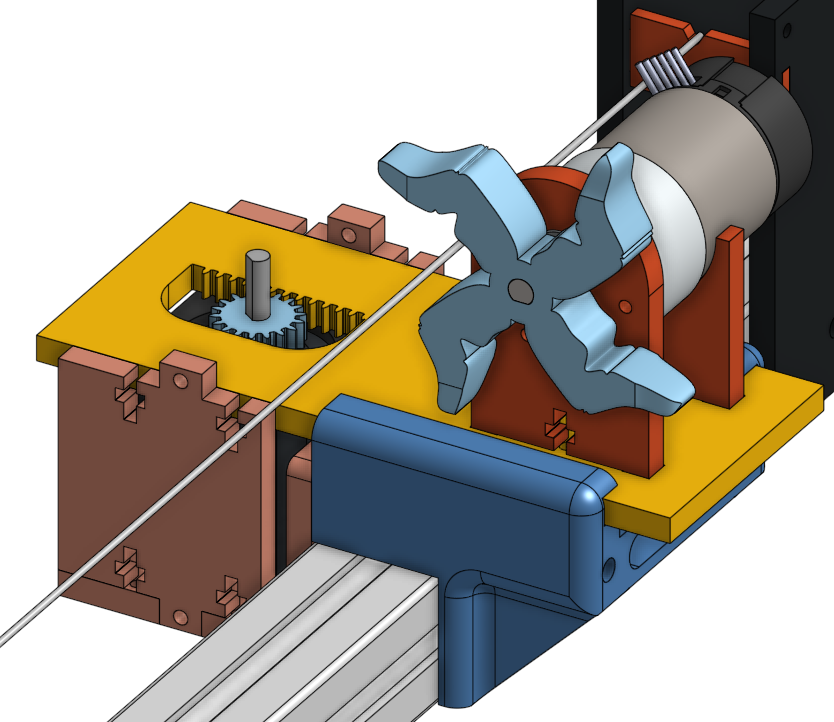
\includegraphics[width=0.6\columnwidth]{PickingMechanism.png}
			\caption{Picking Mechanism}
			\label{fig:picking_mechanism}
		\end{figure}

		Given the requirement for the chordophone to produce multiple volumes of sound, a system that varied the amount of contact between the cord and the picker was designed.
		This causes the pick to displace differing amounts of string resulting in varied oscillation amplitude.
		To achieve this a linear actuator was designed to move the picking motor around the string (see \Cref{fig:picking_mechanism}).
		To pick the string a rotary pickwheel-like mechanism was employed as this has shown success in previously designed chordophone robots \cite{VUW_Chordophones}.

		For this chordophone robot, a linear actuator was used as this provided consistent linear variation and control over the contact area of the pickwheel.
		A linear actuator has been used in previous cordphone robots, however, the size of the mechanism was substatial in size \cite{VUW_Chordophones}.
		As such, this mechanism was designed to be mounted around to the string mount and have a small footprint.
		To achieve this motion a rack and pinion was used, turned by a stepper motor.

		Because the mechanism occupies the space underneath the cord, the pickup has to be placed away from the motors.
		This will reduce the amount of interference with the pickup from the electromagnetic noise generated by the motors.
		It also allows for the pickup to be placed close to the picking zone, with no directly obvious interference from the motors.

		All the pieces aside from one were designed to be laser cut as this is a quick method fo manufacturing, allowing for easy reproduction of the parts to construct this mechanism.
		The piece that cannot be laser cut, can be 3D printed, which makes it easy to reproduce, however it takes longer than the laser cut components.

		Of the two available non-servo motor drivers on the SELCT board, the stepper motors was selected to be used for the rack and pinion as more precise control was required than was offered by the brushed DC motor.
		The stepper motor allows for precise micro stepping which, when travelling a short distance, is important to maintaining the mechanical integrity of the laser cut components.
		The DC motor was then used as it has an attached encoder which allows for both speed control and less precise position control.


	\section{Evaluation}
		\begin{figure}[!h]
			\centering
			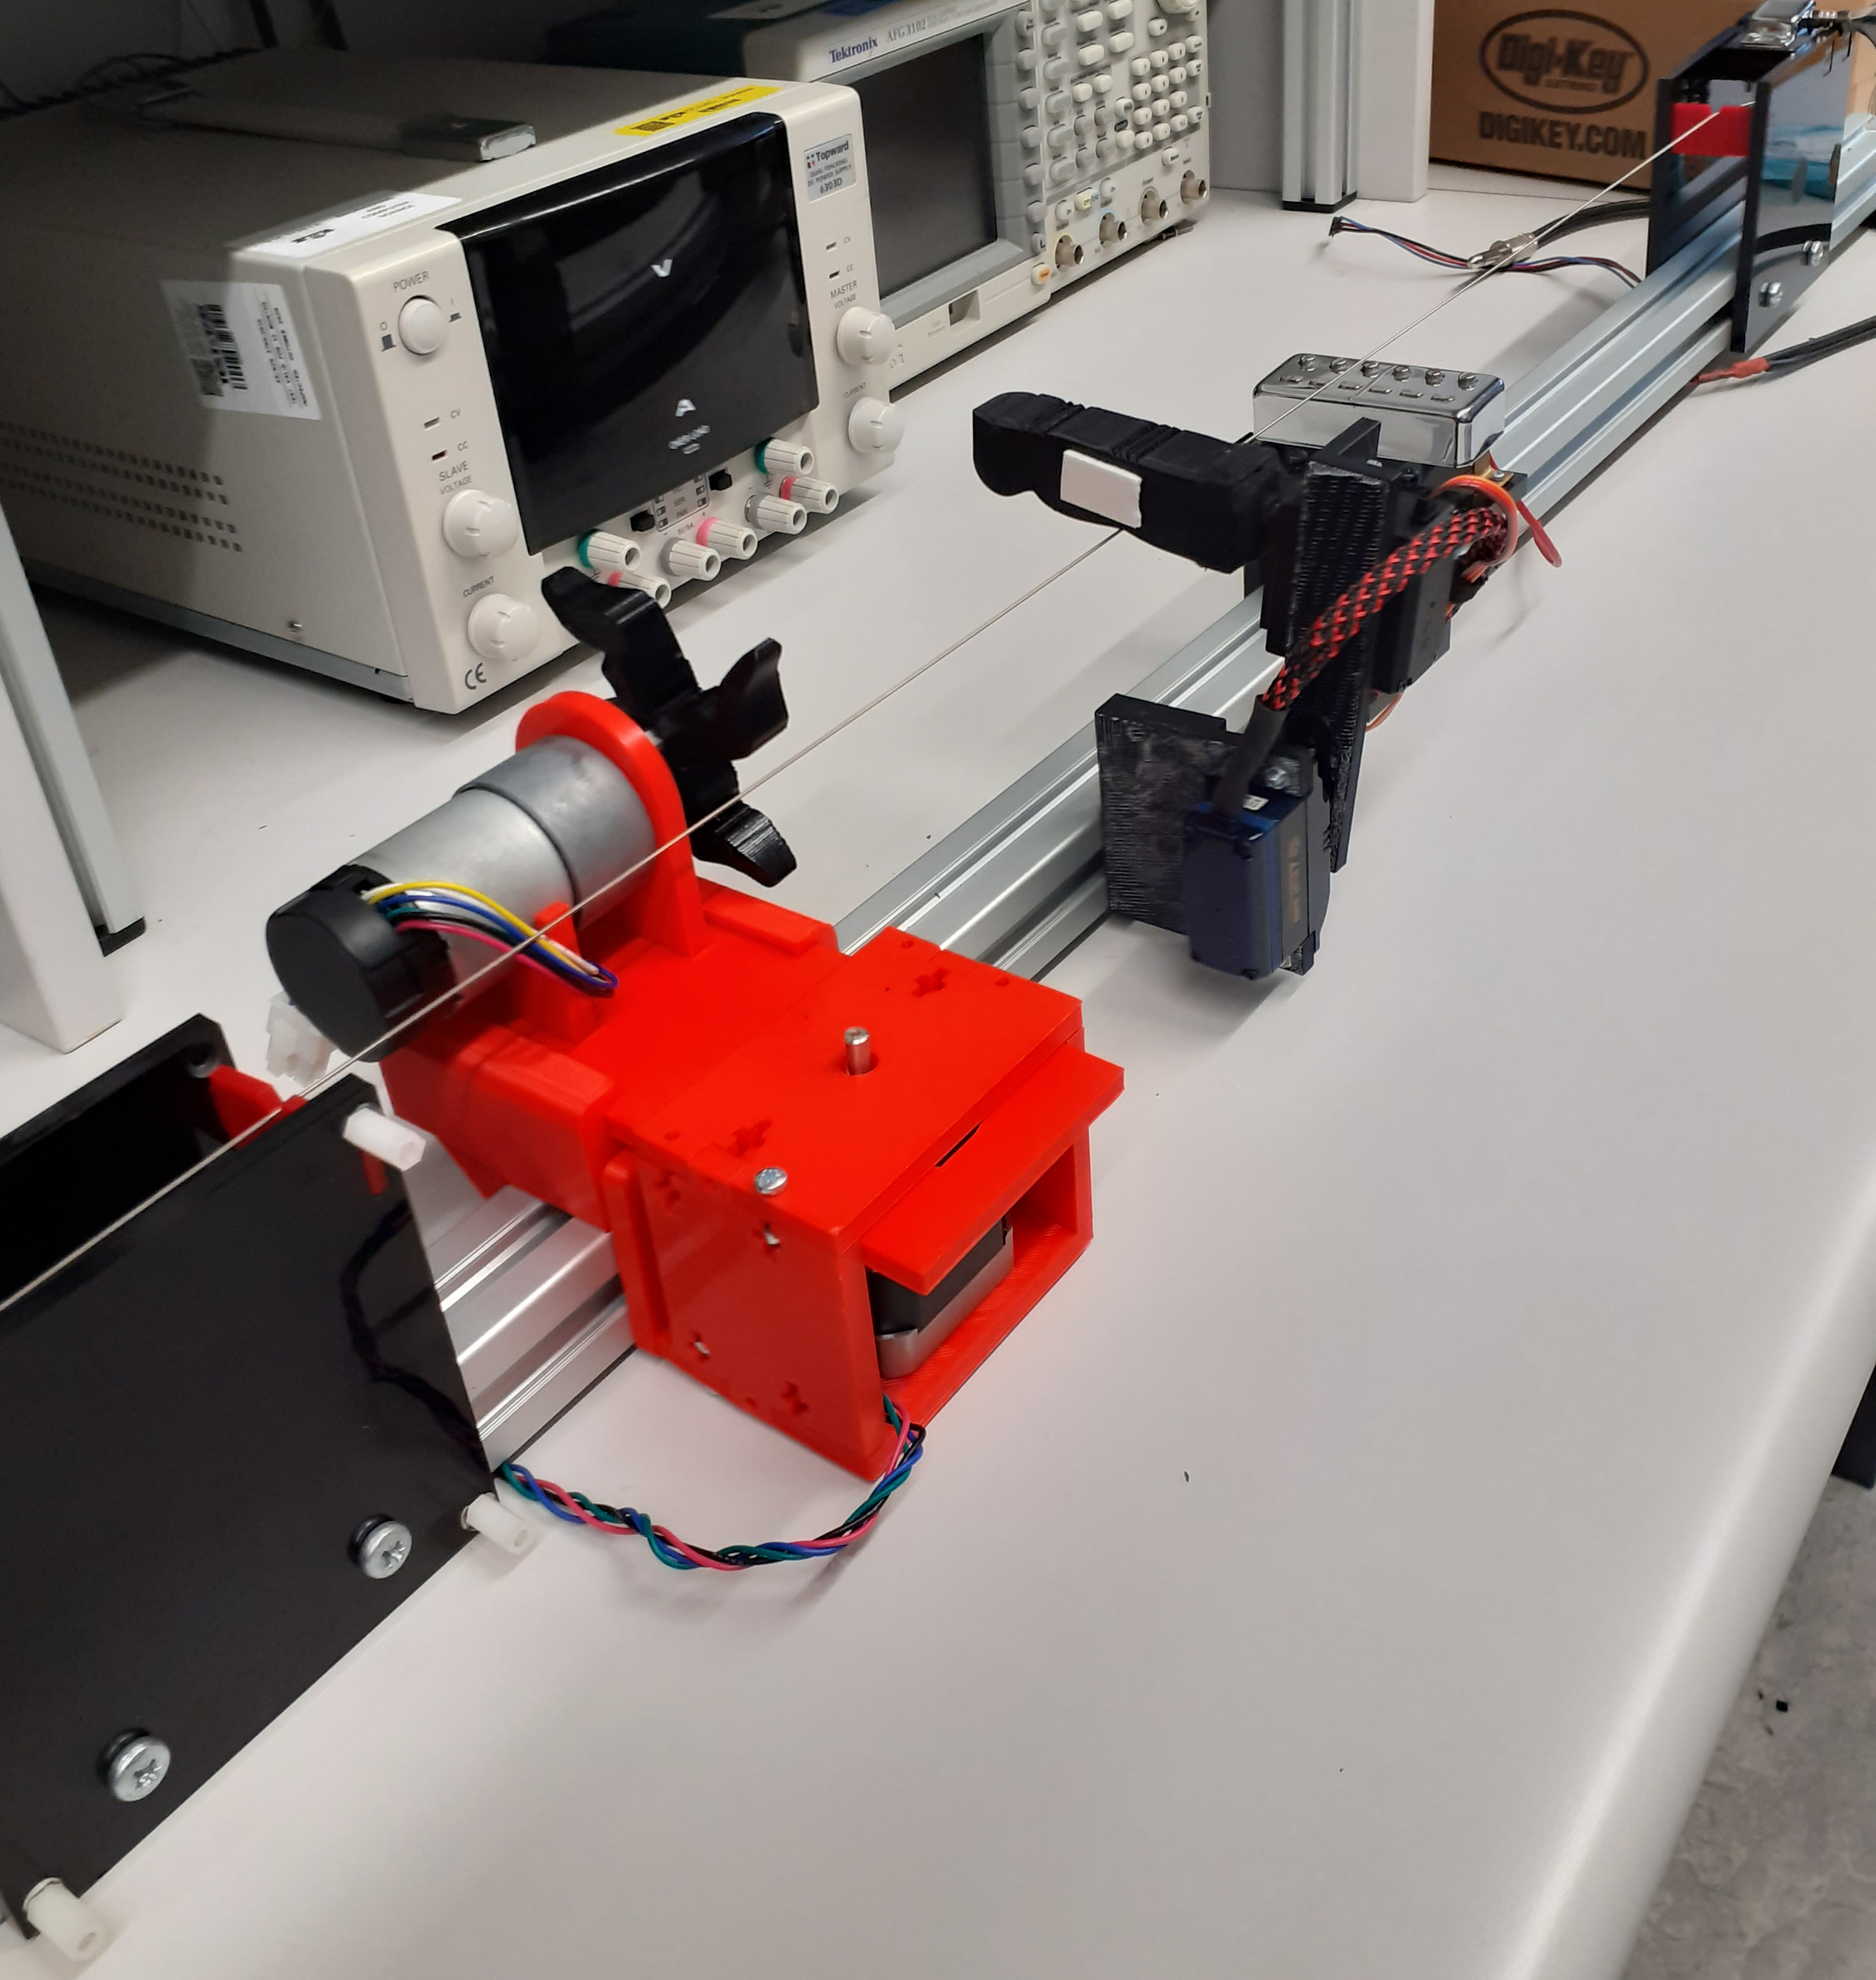
\includegraphics[width=0.6\columnwidth]{finished_chordophone.jpg}
			\caption{Manufactured Chordophone}
			\label{fig:finished}
		\end{figure}
		Evaluation in general was unable to be completed due to entering covid-19 level 4.
		However, the chordophone has been manufactured and assembled (\Cref{fig:finished}) which allowed for physical testing of it, however, no code could be developed to drive it.

		Given time, evaluation of the varying volume would be done by analysing the waveform generated by the pickup and measuring the amplitude of it.
		If the amplitude changed as the stepper motor shifted the motors position to at least 3 different positions, then the mechanisms will have met the design criteria.

		Evaluating the picks per second would be possible by counting the peaks of the waveform created by the pickup.
		These peaks would be the loudest the string would be on a stroke and thus counting every one that was approximately the same height would provide the picks per second.
		To evaluate the damping speed of the damper, an exponential could be fit to the undamped and damped waveforms. This would result in decay rates that are comparable to each other and the target from the requirements.

    \section{Conclusion}
		This paper covered the design and implementation in addition to potential evaluation methods for a chordophone robot.
		While evaluation has not been completed, the physical construction and design has been implemented, allowing for the immediate next steps to be the testing of the system.
		To enable this, a command structure will need to be developed for the midi protocol to allow the changing of materials for both the damping and picking mechanisms as this has not been done in prior chordophone robots.
		In addition to this testing, the additional materials need to be attached to the picking and damping mechanisms to allow for the choice to matter, as currently it is just 3D printed plastic.
		Once the system has been evaluated, this device opens up the possibility for a pick less style of playing to be replicated as the use of silicone to pick the strings is close to the feel of human fingers.

		In terms of the linear actuation, improvements could be made with the design of the rack and pinion gear profiles as they are not fully involute profiles and have a fair amount of backlash.
		Additionally, a similar method that could be explored is the use of a belt driven linear actuator as this constantly engages the stepper motor resulting in less empty movement.
		Further improvements could be made to the size as the stepper motor used in this design is rather large, however, reducing the size of the stepper motor will likely come at the cost of torque or speed.

    \printbibliography

\end{document}